% !TeX program = xelatex
\documentclass[a4paper,10pt]{article}

% ============================================================================
% កញ្ចប់បណ្ណាល័យ (Packages) – តាមលំនាំ NGS Preah Krasang (ls_plan.tex)
% បរិបទ៖ គ្មានស្លាយ LCD និងគ្មានសម្ភារៈកាត់បិទ — ប្រើសន្លឹកកិច្ចការសិស្ស (ស-ខ្មៅ) ជាគោល
% ============================================================================
\usepackage[a4paper, left=0.95cm, right=0.95cm, top=0.85cm, bottom=0.92cm, footskip=0.52cm]{geometry}
\usepackage{amsmath}
\usepackage{unicode-math}
\usepackage{fontspec}
\usepackage{array, longtable, multirow, colortbl}
\usepackage[table]{xcolor}
\usepackage{enumitem}
\usepackage{pifont}
\usepackage{fancyhdr}
\usepackage{tikz}
\usetikzlibrary{calc, arrows.meta, angles, quotes, decorations.markings, decorations.pathreplacing, patterns, babel}

\makeatletter
\let\@expl@@@mark@update@singlecol@structures@@\relax
\makeatother

% ============================================================================
% ការកំណត់ពុម្ពអក្សរ (Fonts Configuration - Cross-Platform Windows + Cloud fonts/)
% ============================================================================
\providecommand{\NGSFindFonts}{%
  \IfFileExists{C:/Windows/Fonts/cambria.ttc}{%
    \def\NGSSysPath{C:/Windows/Fonts/}%
    \def\NGSUserPath{C:/Users/KIT/AppData/Local/Microsoft/Windows/Fonts/}%
  }{%
    \IfFileExists{./fonts/KhmerOSsiemreap.ttf}{\def\NGSSysPath{./fonts/}\def\NGSUserPath{./fonts/}}{%
    \IfFileExists{../fonts/KhmerOSsiemreap.ttf}{\def\NGSSysPath{../fonts/}\def\NGSUserPath{../fonts/}}{%
    \IfFileExists{../../fonts/KhmerOSsiemreap.ttf}{\def\NGSSysPath{../../fonts/}\def\NGSUserPath{../../fonts/}}{%
    \IfFileExists{../../../fonts/KhmerOSsiemreap.ttf}{\def\NGSSysPath{../../../fonts/}\def\NGSUserPath{../../../fonts/}}{%
    \IfFileExists{../../../../fonts/KhmerOSsiemreap.ttf}{\def\NGSSysPath{../../../../fonts/}\def\NGSUserPath{../../../../fonts/}}{%
    \IfFileExists{../../../../../fonts/KhmerOSsiemreap.ttf}{\def\NGSSysPath{../../../../../fonts/}\def\NGSUserPath{../../../../../fonts/}}{%
    \IfFileExists{../../../../../../fonts/KhmerOSsiemreap.ttf}{\def\NGSSysPath{../../../../../../fonts/}\def\NGSUserPath{../../../../../../fonts/}}{%
      \def\NGSSysPath{../../../../../../../fonts/}\def\NGSUserPath{../../../../../../../fonts/}%
    }}}}}}}%
  }%
}
\NGSFindFonts

\setmathfont[Path={\NGSSysPath}, FontIndex=1, Scale=1.02]{cambria.ttc}
\defaultfontfeatures{Ligatures=TeX}

\setmainfont[
  Path={\NGSUserPath}, Extension=.ttf, Script=Khmer,
  BoldFont={KhmerOSsiemreap}, BoldFeatures={FakeBold=1.8},
  ItalicFont={KhmerOSsiemreap}, ItalicFeatures={FakeSlant=0.25},
  BoldItalicFont={KhmerOSsiemreap}, BoldItalicFeatures={FakeBold=1.8, FakeSlant=0.25}
]{KhmerOSsiemreap}

\newfontfamily\muol[Path={\NGSUserPath}, Extension=.ttf, Script=Khmer]{KhmerOSmuollight}
\newfontfamily\TimesEn[Path={\NGSSysPath}, Extension=.ttf, Scale=1.00, BoldFont={timesbd}, ItalicFont={timesi}, BoldItalicFont={timesbi}]{times}
\newfontfamily\NagaBold[Path={\NGSUserPath}, Extension=.ttf]{AKbalthom Naga Bold}
\newfontfamily\CalibriFont[Path={\NGSSysPath}, Extension=.ttf]{calibri}
\newfontfamily\Tacteing[Path={\NGSUserPath}]{TACTENG.TTF}
\newfontfamily\CourierBullet[Path={\NGSSysPath}, Extension=.ttf]{cour}
\newcommand{\wcirc}{{\CourierBullet\fontsize{9.5pt}{11pt}\selectfont o}}

\XeTeXlinebreaklocale "km"
\XeTeXlinebreakskip = 0pt plus 1pt minus 0.1pt

\definecolor{stepgray}{HTML}{D9D9D9}
\definecolor{headgray}{HTML}{F2F2F2}
\definecolor{boxgray}{HTML}{D9D9D9}
\definecolor{darkred}{HTML}{C00000}
\definecolor{red5e}{HTML}{FF0000}

\pagestyle{fancy}
\fancyhf{}
\renewcommand{\headrulewidth}{0pt}
\fancyfoot[R]{\CalibriFont\fontsize{11pt}{13pt}\selectfont\thepage}

\setlength{\parindent}{0pt}
\setlength{\parskip}{0pt}
\setlength{\tabcolsep}{3.8pt}

\newcolumntype{L}[1]{>{\raggedright\arraybackslash}p{#1}}
\newcolumntype{C}[1]{>{\centering\arraybackslash}p{#1}}

\newcommand{\en}[1]{{\TimesEn #1}}
\newcommand{\enbf}[1]{{\TimesEn\textbf{#1}}}
\newcommand{\unit}[1]{\,\text{\en{#1}}}
\newcommand{\fiveE}[1]{{\NagaBold\fontsize{9.5pt}{13pt}\selectfont\textcolor{red5e}{#1}}}
\newcommand{\timenote}[1]{\textcolor{darkred}{\textit{#1}}}
\newcommand{\redsub}[1]{\textcolor{darkred}{#1}}
\newcommand{\graybox}[1]{\colorbox{boxgray}{\strut\hspace{2pt}#1\hspace{2pt}}}
\newcommand{\ditem}{\tikz[baseline=-0.5ex]\fill (0,0.42ex) -- (0.42ex,0) -- (0,-0.42ex) -- (-0.42ex,0) -- cycle;\hspace{0.3em}}
\newcommand{\cnum}[1]{{\fontsize{10.5pt}{12pt}\selectfont\ding{\numexpr181+#1\relax}}\hspace{0.15em}}
\newcommand{\cfig}[1]{\par\vspace{3pt}{\centering #1\par}\vspace{3pt}}
\newcommand{\stepheader}[1]{\multicolumn{3}{|c|}{\cellcolor{stepgray}\muol #1} \\* \noalign{\hrule height 0.4pt}}
\newcommand{\khmflourish}{{\Tacteing\fontsize{36pt}{14pt}\selectfont\raisebox{-5pt}{3}}}

% ============================================================================
% ម៉ាក្រូគូសរូប TikZ ស-ខ្មៅ ១០០% សម្រាប់មេរៀន ២.៤.៤ ស្វ័យគុណនៃ 10 (POW10)
% ============================================================================

% ១. E1 Engage: បេសកកម្មវិក្កយបត្រឃ្លាំងស្រូវ និងដបថ្នាំពេទ្យ
\newcommand{\figEngagePOW}{%
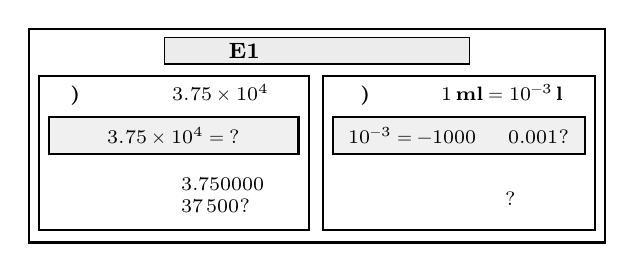
\begin{tikzpicture}[scale=0.92, every node/.style={font=\scriptsize, text=black}]
  \draw[black, line width=0.95pt] (0,0) rectangle (7.95,2.95);
  \node[fill=gray!15, draw=black, line width=0.6pt, inner sep=2pt, font=\footnotesize\bfseries] at (3.975,2.65) {បេសកកម្ម \en{E1}៖ ឃ្លាំងស្រូវ និងដំណក់ថ្នាំពេទ្យ};

  % ឆ្វេង៖ 3.75 x 10^4
  \draw[black, line width=0.8pt] (0.14,0.18) rectangle (3.86,2.30);
  \node[font=\scriptsize\bfseries] at (2.00,2.04) {១) តម្លៃដឹកជញ្ជូន $3.75\times 10^4\text{ ៛}$};
  \draw[black, line width=0.75pt, fill=gray!12] (0.28,1.22) rectangle (3.72,1.74);
  \node at (2.00,1.48) {$3.75\times 10^4 = ?$};
  \node[align=center] at (2.00,0.66) {តើថែមសូន្យ ៤ បាន $3.750000$\\ឬរំកិលក្បៀសបាន $37\,500$?};

  % ស្ដាំ៖ 10^{-3} L
  \draw[black, line width=0.8pt] (4.06,0.18) rectangle (7.81,2.30);
  \node[font=\scriptsize\bfseries] at (5.935,2.04) {២) ចំណុះថ្នាំ $1\unit{ml} = 10^{-3}\unit{l}$};
  \draw[black, line width=0.75pt, fill=gray!12] (4.20,1.22) rectangle (7.67,1.74);
  \node at (5.935,1.48) {$10^{-3} = -1000$ \;ឬ\; $0.001$?};
  \node[align=center] at (5.935,0.66) {តើនិទស្សន្តដកធ្វើឱ្យចំនួន\textbf{អវិជ្ជមាន}\\ឬជា\textbf{ទសភាគតូចវិជ្ជមាន}?};
\end{tikzpicture}}

% ២. E2 POE 1: ជណ្ដើរឆ្លុះស្វ័យគុណនៃ 10 (10^2 <-> 10^0 <-> 10^{-2})
\newcommand{\figLadderPOW}{%
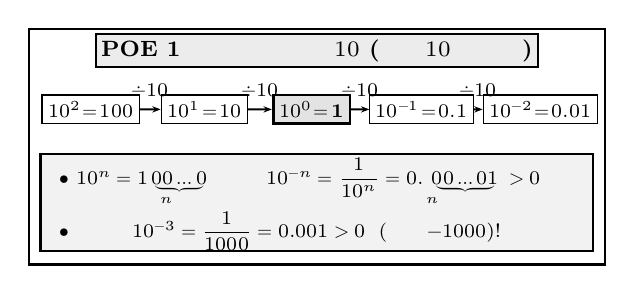
\begin{tikzpicture}[scale=0.92, every node/.style={font=\scriptsize, text=black}]
  \draw[black, line width=0.95pt] (0,0) rectangle (7.95,3.25);
  \node[fill=gray!15, draw=black, line width=0.6pt, inner sep=2pt, font=\footnotesize\bfseries] at (3.975,2.95) {\en{POE 1}៖ ជណ្ដើរឆ្លុះស្វ័យគុណនៃ $10$ (ចែកនឹង $10$ ម្ដងមួយកាំ)};

  \node[draw=black, fill=white, inner sep=2.2pt] (P2) at (0.85,2.14) {$10^2\!=\!100$};
  \node[draw=black, fill=white, inner sep=2.2pt] (P1) at (2.42,2.14) {$10^1\!=\!10$};
  \node[draw=black, fill=gray!22, line width=0.95pt, inner sep=2.2pt] (P0) at (3.90,2.14) {$10^0\!=\!\mathbf{1}$};
  \node[draw=black, fill=white, inner sep=2.2pt] (N1) at (5.42,2.14) {$10^{-1}\!=\!0.1$};
  \node[draw=black, fill=white, inner sep=2.2pt] (N2) at (7.06,2.14) {$10^{-2}\!=\!0.01$};

  \draw[black, line width=0.7pt, -{Stealth[length=3pt]}] (P2) -- node[above=1pt]{$\div 10$} (P1);
  \draw[black, line width=0.7pt, -{Stealth[length=3pt]}] (P1) -- node[above=1pt]{$\div 10$} (P0);
  \draw[black, line width=0.7pt, -{Stealth[length=3pt]}] (P0) -- node[above=1pt]{$\div 10$} (N1);
  \draw[black, line width=0.7pt, -{Stealth[length=3pt]}] (N1) -- node[above=1pt]{$\div 10$} (N2);

  \draw[black, line width=0.8pt, fill=gray!10] (0.16,0.18) rectangle (7.79,1.52);
  \node[anchor=west] at (0.28,1.15) {$\bullet$ $10^n = 1\underbrace{00\dots 0}_{n\text{ សូន្យ}}$ \quad ឯ \quad $10^{-n} = \dfrac{1}{10^n} = 0.\underbrace{00\dots 01}_{n\text{ ខ្ទង់ក្រោយក្បៀស}} > 0$};
  \node[anchor=west] at (0.28,0.46) {$\bullet$ \textbf{ប្រយ័ត្ន៖} $10^{-3} = \dfrac{1}{1000} = 0.001 > 0$ \;(\textbf{មិនមែន} $-1000$)!};
\end{tikzpicture}}

% ៣. E2 POE 2: ផ្លូវលោតក្បៀសស្ដាំ-ឆ្វេង (Decimal-Hop Track)
\newcommand{\figHopTrackPOW}{%
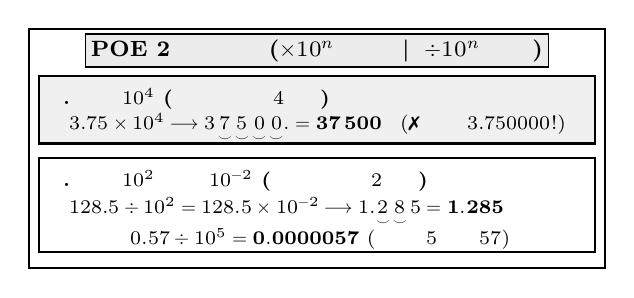
\begin{tikzpicture}[scale=0.92, every node/.style={font=\scriptsize, text=black}]
  \draw[black, line width=0.95pt] (0,0) rectangle (7.95,3.30);
  \node[fill=gray!15, draw=black, line width=0.6pt, inner sep=2pt, font=\footnotesize\bfseries] at (3.975,3.00) {\en{POE 2}៖ ធ្នូលោតក្បៀស ($\times 10^n$ ទៅស្ដាំ \;\textbar\; $\div 10^n$ ទៅឆ្វេង)};

  % ជួរលើ៖ 3.75 x 10^4
  \draw[black, line width=0.85pt, fill=gray!12] (0.14,1.72) rectangle (7.81,2.65);
  \node[anchor=west] at (0.26,2.34) {\textbf{ក. គុណនឹង $10^4$ (រំកិលក្បៀសទៅស្ដាំ $4$ ខ្ទង់)៖}};
  \node[anchor=west] at (0.42,1.94) {$3.75 \times 10^4 \longrightarrow 3\,\underset{\smile}{7}\,\underset{\smile}{5}\,\underset{\smile}{0}\,\underset{\smile}{0}. = \mathbf{37\,500}$ \;\;(\ding{55} មិនមែន $3.750000$!)};

  % ជួរក្រោម៖ 128.5 / 10^2
  \draw[black, line width=0.85pt] (0.14,0.22) rectangle (7.81,1.52);
  \node[anchor=west] at (0.26,1.20) {\textbf{ខ. ចែកនឹង $10^2$ ឬគុណនឹង $10^{-2}$ (រំកិលក្បៀសទៅឆ្វេង $2$ ខ្ទង់)៖}};
  \node[anchor=west] at (0.42,0.78) {$128.5 \div 10^2 = 128.5 \times 10^{-2} \longrightarrow 1.\underset{\smile}{2}\,\underset{\smile}{8}\,5 = \mathbf{1.285}$};
  \node[anchor=west] at (0.42,0.40) {ដូចគ្នានឹង $0.57 \div 10^5 = \mathbf{0.0000057}$ (ថែមសូន្យ $5$ ពីមុខ $57$)};
\end{tikzpicture}}

% ៤. E3/E4: ស្ពានប្ដូរខ្នាតប្រព័ន្ធម៉ែត្រ (Metric Bridge cm->m, g->kg, ml->l)
\newcommand{\figMetricBridgePOW}{%
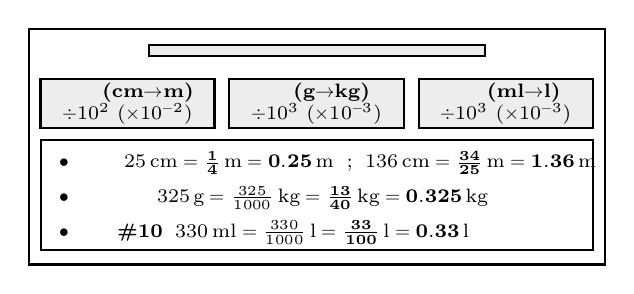
\begin{tikzpicture}[scale=0.92, every node/.style={font=\scriptsize, text=black}]
  \draw[black, line width=0.95pt] (0,0) rectangle (7.95,3.25);
  \node[fill=gray!15, draw=black, line width=0.6pt, inner sep=2pt, font=\footnotesize\bfseries] at (3.975,2.95) {ស្ពានប្ដូរខ្នាតប្រព័ន្ធម៉ែត្រជាប្រភាគសម្រួល និងទសភាគ};

  \draw[black, line width=0.8pt, fill=gray!14] (0.16,1.88) rectangle (2.56,2.56);
  \node[align=center] at (1.36,2.22) {\textbf{ប្រវែង (\en{cm}$\to$\en{m})}\\$\div 10^2$ ($\times 10^{-2}$)};

  \draw[black, line width=0.8pt, fill=gray!14] (2.76,1.88) rectangle (5.18,2.56);
  \node[align=center] at (3.97,2.22) {\textbf{ម៉ាស (\en{g}$\to$\en{kg})}\\$\div 10^3$ ($\times 10^{-3}$)};

  \draw[black, line width=0.8pt, fill=gray!14] (5.38,1.88) rectangle (7.79,2.56);
  \node[align=center] at (6.585,2.22) {\textbf{ចំណុះ (\en{ml}$\to$\en{l})}\\$\div 10^3$ ($\times 10^{-3}$)};

  \draw[black, line width=0.75pt] (0.16,0.20) rectangle (7.79,1.72);
  \node[anchor=west] at (0.28,1.40) {$\bullet$ \textbf{គំរូ ២៖} $25\unit{cm} = \mathbf{\frac{1}{4}\unit{m}} = \mathbf{0.25\unit{m}}$ \;;\; $136\unit{cm} = \mathbf{\frac{34}{25}\unit{m}} = \mathbf{1.36\unit{m}}$};
  \node[anchor=west] at (0.28,0.92) {$\bullet$ \textbf{ប្រតិបត្តិ ២៖} $325\unit{g} = \frac{325}{1000}\unit{kg} = \mathbf{\frac{13}{40}\unit{kg}} = \mathbf{0.325\unit{kg}}$};
  \node[anchor=west] at (0.28,0.44) {$\bullet$ \textbf{លំហាត់ \#10៖} $330\unit{ml} = \frac{330}{1000}\unit{l} = \mathbf{\frac{33}{100}\unit{l}} = \mathbf{0.33\unit{l}}$};
\end{tikzpicture}}

% ៥. E5 Diagnostic Options A-D
\newcommand{\figExitCardsPOW}{%
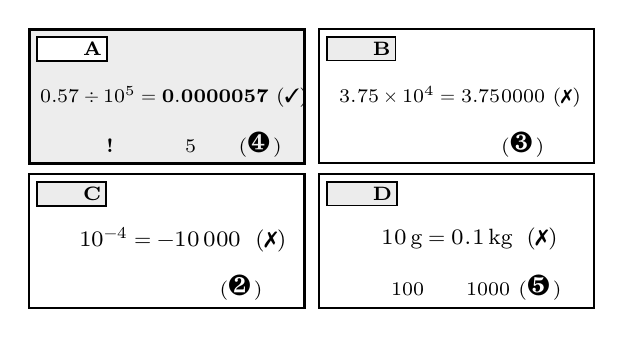
\begin{tikzpicture}[scale=0.92, every node/.style={font=\scriptsize, text=black}]
  \draw[black, line width=1.1pt, fill=gray!14] (0,2.00) rectangle (3.80,3.85);
  \node[anchor=north west, fill=white, draw=black, line width=0.6pt, inner sep=1.8pt] at (0.10,3.75) {\textbf{ជម្រើស \en{A}}};
  \node at (2.00,2.92) {$0.57\div 10^5 = \mathbf{0.0000057}$ (\ding{51})};
  \node at (1.90,2.25) {\textbf{ត្រឹមត្រូវ!} រំកិលឆ្វេង $5$ ខ្ទង់ (\cnum{4})};

  \draw[black, line width=0.9pt] (4.00,2.00) rectangle (7.80,3.85);
  \node[anchor=north west, fill=gray!15, draw=black, line width=0.6pt, inner sep=1.8pt] at (4.10,3.75) {\textbf{ជម្រើស \en{B}}};
  \node at (5.95,2.92) {$3.75\times 10^4 = 3.750000$ (\ding{55})};
  \node at (5.90,2.25) {អន្ទាក់ថែមសូន្យចុងទសភាគ (\cnum{3})};

  \draw[black, line width=0.9pt] (0,0) rectangle (3.80,1.85);
  \node[anchor=north west, fill=gray!15, draw=black, line width=0.6pt, inner sep=1.8pt] at (0.10,1.75) {\textbf{ជម្រើស \en{C}}};
  \node[font=\footnotesize] at (2.12,0.95) {$10^{-4} = -10\,000$ \;(\ding{55})};
  \node at (1.90,0.28) {ច្រឡំនិទស្សន្តដកនឹងចំនួនដក (\cnum{2})};

  \draw[black, line width=0.9pt] (4.00,0) rectangle (7.80,1.85);
  \node[anchor=north west, fill=gray!15, draw=black, line width=0.6pt, inner sep=1.8pt] at (4.10,1.75) {\textbf{ជម្រើស \en{D}}};
  \node[font=\footnotesize] at (6.08,0.95) {$10\unit{g} = 0.1\unit{kg}$ \;(\ding{55})};
  \node at (5.90,0.28) {ចែកនឹង $100$ ជំនួស $1000$ (\cnum{5})};
\end{tikzpicture}}

\begin{document}
\fontsize{10pt}{15.2pt}\selectfont

% -------------------- ក្បាលកិច្ចតែងការ --------------------
\begin{center}
  {\muol\fontsize{11pt}{16pt}\selectfont ព្រះរាជាណាចក្រកម្ពុជា}\\[2pt]
  {\muol\fontsize{10pt}{15pt}\selectfont ជាតិ សាសនា ព្រះមហាក្សត្រ}\\[1pt]
  \khmflourish
\end{center}

\vspace{-24pt}
{\muol\fontsize{9.5pt}{12.5pt}\selectfont
មន្ទីរអប់រំ យុវជន និងកីឡា ខេត្តកំពង់ធំ\\
ការិយាល័យអប់រំ យុវជន និងកីឡា ស្រុកកំពង់ស្វាយ\\
អនុវិទ្យាល័យព្រះក្រសាំង}

\vspace{1pt}
\begin{center}
  {\muol\fontsize{10pt}{14pt}\selectfont កិច្ចតែងការបង្រៀន}
\end{center}
\vspace{0pt}

% -------------------- ព័ត៌មានទូទៅ --------------------
{\renewcommand{\arraystretch}{0.98}
\hspace*{3.1cm}%
\begin{tabular}{@{}l l L{11.0cm}@{}}
  - \hspace{0.35cm} មុខវិជ្ជា & : & គណិតវិទ្យា ថ្នាក់ទី៨ (ពីជគណិត) \\
  - \hspace{0.35cm} ចំណងជើងមេរៀន & : & មេរៀនទី២៖ ស្វ័យគុណ \\
  - \hspace{0.35cm} ចំណងជើងរង & : & ៤.៤. ស្វ័យគុណនៃ \en{10} (សៀវភៅពុម្ព ទំ.១៩–២១ និងលំហាត់ \#10 ទំ.២៦) \\
  - \hspace{0.35cm} រយៈពេល & : & ១ ម៉ោងសិក្សា (៥០ នាទី) \\
  - \hspace{0.35cm} បង្រៀនដោយ & : & ហុក ប៊ុនថែន \\
  - \hspace{0.35cm} កាលបរិច្ឆេទ & : & ថ្ងៃអង្គារ ទី១៧ ខែវិច្ឆិកា ឆ្នាំ២០២៦ \\
\end{tabular}

\vspace{2pt}

% -------------------- I. វត្ថុបំណង --------------------
\textbf{I.} {\muol វត្ថុបំណង}\\[1pt]
\hspace*{0.55cm}%
\begin{tabular}{@{}l l L{14.2cm}@{}}
  \wcirc \hspace{0.25cm} វិជ្ជាសម្បទា & : & សិស្សប្រាប់ទម្រង់ទូទៅនៃស្វ័យគុណគោលដប់ $10^n = 1\underbrace{00\dots 0}_{n\text{ សូន្យ}}$, $10^0=1$, និង $10^{-n} = \frac{1}{10^n} = 0.\underbrace{00\dots 01}_{n\text{ ខ្ទង់}}$ ($n\in\mathbb{Z}^+$) ព្រមទាំងក្បួនរំកិលក្បៀសពេលគុណ ឬចែកចំនួនទសភាគនឹង $10^n$ ។ \\
  \wcirc \hspace{0.25cm} បំណិនសម្បទា & : & សិស្សគូសធ្នូលោតក្បៀសលើសន្លឹកកិច្ចការដើម្បីគណនាផលគុណ-ផលចែកទសភាគនឹង $10^n$ និងប្ដូរខ្នាតប្រវែង (\en{cm}$\to$\en{m}) ម៉ាស (\en{g}$\to$\en{kg}) ចំណុះ (\en{ml}$\to$\en{l}) ជាប្រភាគសម្រួល និងទសភាគបានត្រឹមត្រូវ ។ \\
  \wcirc \hspace{0.25cm} ចរិយាសម្បទា & : & សិស្សមានភាពហ្មត់ចត់ក្នុងការរាប់ខ្ទង់ក្បៀស ចៀសវាងអន្ទាក់ថែមសូន្យចុងទសភាគ ឬច្រឡំ $10^{-n}$ ថាជាចំនួនអវិជ្ជមាន និងសហការផ្ទៀងផ្ទាត់ខ្នាតក្នុងជីវភាពរស់នៅជាដៃគូ ។ \\
\end{tabular}

\vspace{2pt}

% -------------------- II. សម្ភារៈឧបទេស --------------------
\textbf{II.} {\muol សម្ភារៈឧបទេស}\\[1pt]
\hspace*{0.55cm}$\bullet$ \hspace{0.35cm} សៀវភៅសិក្សាគោលគណិតវិទ្យាថ្នាក់ទី៨ (ទំ.១៩–២១, ២៦) ក្ដារខៀន ដីស បន្ទាត់ម៉ែត្រក្ដារខៀន និងសន្លឹកកិច្ចការសិស្ស ស-ខ្មៅ (\en{Worksheet\_POW10} ទំព័រ ១–២ សម្រាប់បំពេញផ្ទាល់ គ្មានស្លាយ \en{LCD})

\vspace{2pt}

% -------------------- III. វិធីសាស្រ្តបង្រៀន --------------------
\textbf{III.} {\muol វិធីសាស្រ្តបង្រៀន}\\[1pt]
\hspace*{0.45cm}%
\begin{tabular}{@{}l l L{14.85cm}@{}}
  $\bullet$ \hspace{0.25cm} គោលវិធី & : & សិស្សមជ្ឈមណ្ឌល (បង្រៀនតាមសន្លឹកកិច្ចការស៊ើបអង្កេត និងក្ដារខៀន គ្មាន \en{LCD}) \\
  $\bullet$ \hspace{0.25cm} យុទ្ធវិធីបង្រៀន & : & គំរូ \en{5Es} រួមបញ្ចូលជណ្ដើរឆ្លុះតម្លៃខ្ទង់ (\en{Symmetric Place-Value Ladder}), ផ្លូវធ្នូលោតក្បៀស (\en{Decimal-Hop Track}), និងស្ពានប្ដូរខ្នាតប្រព័ន្ធម៉ែត្រជាប្រភាគ-ទសភាគ \\
\end{tabular}
}

\vspace{2pt}

% -------------------- IV. ដំណើរការបង្រៀន --------------------
\textbf{IV.} {\muol ដំណើរការបង្រៀន}

\vspace{1pt}

\renewcommand{\arraystretch}{1.15}
\begin{longtable}{|L{5.50cm}|L{7.90cm}|L{4.80cm}|}
\hline
\rowcolor{headgray}
\multicolumn{1}{|c|}{\muol សកម្មភាពគ្រូ} &
\multicolumn{1}{c|}{\muol ខ្លឹមសារមេរៀន} &
\multicolumn{1}{c|}{\muol សកម្មភាពសិស្ស} \\
\hline
\endfirsthead
\hline
\endhead
\hline
\endfoot
\hline
\endlastfoot

% ==================== ជំហានទី១ (2min) ====================
\stepheader{ជំហានទី១ \enbf{(}រដ្ឋបាលថ្នាក់\enbf{)}}
$\bullet$ ពិនិត្យអវត្តមាន អនាម័យ និងសណ្ដាប់ធ្នាប់ថ្នាក់រៀន
&
$\bullet$ រដ្ឋបាលថ្នាក់ និងការរៀបចំដៃគូសិក្សា (២ នាក់ក្នុង ១ តុ)
&
$\circ$ ប្រធានថ្នាក់រាយការណ៍អវត្តមាន \\[3pt]

$\bullet$ ចែក \textbf{សន្លឹកកិច្ចការសិស្ស (\en{Worksheet\_POW10})} ម្នាក់ ១ សន្លឹក (ផ្កាប់ទុកសិន)
&
$\bullet$ សន្លឹកកិច្ចការសិស្ស ស-ខ្មៅ (\en{Worksheet\_POW10} ទំព័រ ១–២)
&
$\circ$ ទទួលសន្លឹកកិច្ចការ និងត្រៀមប៊ិច/ខ្មៅដៃ \\
\hline

% ==================== ជំហានទី២ (9min: <=3 + 3 + E1 3) ====================
\stepheader{ជំហានទី២ \enbf{(}កិច្ចការផ្ទះ \enbf{+} ទំនាក់ទំនងមេរៀនថ្មី\enbf{)}}
\ditem \textbf{កំណែកិច្ចការផ្ទះ ($\le 3\unit{min}$)} \timenote{(កុំសរសេរវែង)} \par
$\bullet$ ហៅសិស្ស ២ នាក់ឡើងកែលំហាត់ម៉ោងមុន (៤.៣ ស្វ័យគុណនៃផលចែក និងនិទស្សន្តដក)
&
{\centering\redsub{កំណែកិច្ចការផ្ទះមេរៀនមុន (៤.៣)}\par} \par
$\bullet$ \textbf{ក.} $\left(\dfrac{1}{10}\right)^3 = \dfrac{1^3}{10^3} = \dfrac{1}{1000} = 10^{-3}$ \par
$\bullet$ \textbf{ខ.} $\dfrac{10^2}{10^5} = 10^{2-5} = 10^{-3}$ \;និង\; $10^0 = 1$
&
$\circ$ ផ្ទៀងផ្ទាត់ច្បាប់ $a^{-n} = \dfrac{1}{a^n}$ និង $a^0 = 1$ \\[3pt]

\ditem \textbf{រំលឹកមេរៀនទាក់ទង (3min)} \par
$\bullet$ សួររំលឹកចំណេះដឹងថ្នាក់ទី៧ អំពីការគុណ និងចែកទសភាគនឹង $10,\; 100$
&
{\centering\redsub{រំលឹកមេរៀនទាក់ទងមេរៀនថ្មី}\par} \par
$\bullet$ $3.75 \times 10 = 37.5$ \; ; \; $3.75 \times 100 = 375$ \par
$\bullet$ $25 \div 100 = \dfrac{25}{100} = \dfrac{1}{4} = 0.25$ (សម្រួលនឹង $25$)
&
$\circ$ ឆ្លើយរហ័សអំពីការរំកិលក្បៀស និងសម្រួលប្រភាគ \\[3pt]

\fiveE{E1 - Engage (3min)} \timenote{(កុំទាន់ផ្ដល់ចម្លើយ)} \par
\ditem \textbf{«បេសកកម្មវិក្កយបត្រឃ្លាំងស្រូវ និងដំណក់ថ្នាំពេទ្យ»} \par
$\bullet$ ឱ្យសិស្សបើកសន្លឹកកិច្ចការទំព័រ ១ គូសធីកទស្សន៍ទាយលើសំណួរ ២
&
{\centering\redsub{បេសកកម្ម E1៖ ឃ្លាំងស្រូវ និងដំណក់ថ្នាំពេទ្យ}\par} \par
$\bullet$ \textbf{សំណួរ ១៖} $3.75 \times 10^4$ ស្មើ $3.750000$ ឬស្មើ $37\,500$? \par
$\bullet$ \textbf{សំណួរ ២៖} តើ $10^{-3}\unit{l}$ ($1\unit{ml}$) ស្មើ $-1000$ ឬ $0.001$?
&
$\circ$ គូសធីកទស្សន៍ទាយលើសន្លឹកកិច្ចការទំព័រ ១ \\[3pt]

&
\cfig{\figEngagePOW}
& \\[3pt]

$\bullet$ កត់ចំនួនដៃសិស្សជ្រើសរើសទុកនៅជ្រុងក្ដារខៀន សម្រាប់ផ្ទៀងនៅវគ្គ \en{E5}
&
$\bullet$ ស្ថិតិទស្សន៍ទាយ៖ ថែមសូន្យចុងទសភាគ ទល់នឹង រំកិលក្បៀស ; ចំនួនដក ទល់នឹង ទសភាគតូចវិជ្ជមាន
&
$\circ$ លើកដៃបង្ហាញការទស្សន៍ទាយ និងត្រៀមរុករក \\
\hline

% ==================== ជំហានទី៣ (17min: E2 11m + E3 6m) ====================
\stepheader{ជំហានទី៣ \enbf{(}ខ្លឹមសារមេរៀនថ្មី\enbf{)}}
\fiveE{E2 - Explore (11min)} \par
$\bullet$ សរសេរចំណងជើងរងលើក្ដារខៀន
&
\textbf{៤.៤. ស្វ័យគុណនៃ \en{10}} (សៀវភៅពុម្ព ទំ.១៩–២១)
&
$\circ$ កត់ចំណងជើងចូលសៀវភៅ \\[3pt]

\ditem \textbf{សកម្មភាព ១៖ ជណ្ដើរឆ្លុះស្វ័យគុណនៃ $10$ \en{POE 1} (6min, ផ្នែកទី១-ក)} \par
$\bullet$ ឱ្យដៃគូបំពេញតារាងស្វ័យគុណវិជ្ជមាន ($10^1..10^7$) និងស្វ័យគុណអវិជ្ជមាន ($10^{-1}..10^{-7}$) ដោយចែកនឹង $10$ ម្ដងមួយកាំ (ទំ.១៩–២០)
&
{\centering\textbf{សកម្មភាព ១ (\en{POE 1})៖ លំនាំសូន្យនៃ $10^n$ និង $10^{-n}$}\par} \par
$\bullet$ $10^1=10,\; 10^2=100,\; 10^3=1000,\dots,\; 10^7=10\,000\,000$ \par
$\bullet$ $10^0=1 \xrightarrow{\div 10} 10^{-1}=\dfrac{1}{10}=0.1,\; 10^{-2}=\dfrac{1}{100}=0.01,\; 10^{-3}=0.001,\dots,\; 10^{-7}=0.0000001$
&
$\circ$ បំពេញតារាងជណ្ដើរឆ្លុះលើសន្លឹកកិច្ចការ និងរាប់ចំនួនខ្ទង់ \\[3pt]

&
\cfig{\figLadderPOW}
& \\[3pt]

\hspace*{0.3em}– \textbf{សំណួរ៖} «ក្នុង $10^{-4}=0.0001$ តើមានប៉ុន្មានខ្ទង់ក្រោយក្បៀស? តើវាតូចជាង $0$ ឬធំជាង $0$?»
&
$\bullet$ \textbf{សន្និដ្ឋានរុករក ១៖} $10^{-4}=0.0001 > 0$ មាន \textbf{$4$ ខ្ទង់ក្រោយក្បៀស} (សូន្យ $3$ ពីក្រោយក្បៀស + លេខ $1$) មិនមែនចំនួនអវិជ្ជមានឡើយ!
&
$\circ$ ឆ្លើយសំណួរ និងកត់សន្និដ្ឋានលើសន្លឹកកិច្ចការ \\[3pt]

\ditem \textbf{សកម្មភាព ២៖ ផ្លូវធ្នូលោតក្បៀស \en{POE 2} (5min, ផ្នែកទី១-ខ)} \par
$\bullet$ ឱ្យសិស្សគណនា \textbf{ឧទាហរណ៍ ក. ទំ.២០} ($3.75\times 10^4$) ដោយបំបែក $10^4=10\,000$ រួចគូសធ្នូលោតក្បៀសទៅស្ដាំ
&
{\centering\textbf{សកម្មភាព ២ (\en{POE 2})៖ ឧទាហរណ៍ ទំ.២០}\par} \par
$\bullet$ \textbf{ក.} $3.75\times 10^4 = 3.75\times 10\,000 = 37\,500$ (លោតស្ដាំ $4$ ខ្ទង់ — ថែមសូន្យ $2$ ខ្ទង់)
&
$\circ$ គូសធ្នូលោតក្បៀសទៅស្ដាំ $4$ ខ្ទង់ និងផ្ទៀងនឹងការគុណផ្ទាល់ \\[3pt]

$\bullet$ ឱ្យសិស្សបន្តគណនា \textbf{ឧទាហរណ៍ ខ. ទំ.២០} ($128.5\div 10^2$) ដោយប្រៀបធៀបនឹងការគុណនឹង $10^{-2}$
&
$\bullet$ \textbf{ខ.} $128.5\div 10^2 = \dfrac{128.5}{100} = 128.5\times 10^{-2} = 1.285$ (លោតឆ្វេង $2$ ខ្ទង់)
&
$\circ$ គូសធ្នូលោតក្បៀសទៅឆ្វេង $2$ ខ្ទង់លើសន្លឹកកិច្ចការ \\[3pt]

&
\cfig{\figHopTrackPOW}
& \\[3pt]

% --- E3 Explain (6min) ---
\fiveE{E3 - Explain (6min)} \par
\ditem \textbf{សំយោគក្បួន «ជាទូទៅ» ទំ.១៩–២០ និងធនាគារហេតុផល (ផ្នែកទី២)} \par
$\bullet$ ឱ្យតំណាងដៃគូបង្គុំប្រអប់ \textbf{ជាទូទៅ ទី១ (ទំ.១៩–២០)} និង \textbf{ជាទូទៅ ទី២ (ទំ.២០)}
&
$\bullet$ \textbf{ជាទូទៅ ១ (ទំ.១៩–២០)៖} ចំពោះ $n\in\mathbb{Z}^+$៖ \par
{\centering\graybox{$10^n = 1\underbrace{00\dots 0}_{\text{សូន្យ }n}$ \quad និង \quad $10^{-n} = \dfrac{1}{10^n} = 0.\underbrace{00\dots 01}_{n\text{ ខ្ទង់}}$}\par}
$\bullet$ \textbf{ជាទូទៅ ២ (ទំ.២០)៖} គុណនឹង $10^n \to$ រំកិលក្បៀសទៅ\textbf{ស្ដាំ} $n$ ខ្ទង់ ; ចែកនឹង $10^n$ (ឬគុណនឹង $10^{-n}$) $\to$ រំកិលក្បៀសទៅ\textbf{ឆ្វេង} $n$ ខ្ទង់ ។
&
$\circ$ បំពេញប្រអប់ «ជាទូទៅ» ទាំង ២ ក្នុងសន្លឹកកិច្ចការ \\[3pt]

$\bullet$ សង្ខេប \textbf{ធនាគារហេតុផល \cnum{1}--\cnum{5}} ភ្ជាប់នឹងការប្ដូរខ្នាតម៉ែត្រ
&
\textbf{ធនាគារហេតុផល \en{B\&W} (\cnum{1}--\cnum{5})៖} \par
\cnum{1} ស្វ័យគុណវិជ្ជមាន៖ $10^n = 1\underbrace{00\dots 0}_{n\text{ សូន្យ}}$ និង $10^0 = 1$ \par
\cnum{2} ស្វ័យគុណអវិជ្ជមាន៖ $10^{-n} = \frac{1}{10^n} = 0.\underbrace{00\dots 01}_{n\text{ ខ្ទង់}} > 0$ (មិនអវិជ្ជមាន!) \par
\cnum{3} គុណនឹង $10^n$ ($n>0$)៖ រំកិលក្បៀសទៅ\textbf{ស្ដាំ} $n$ ខ្ទង់ (ថែម $0$ បើខ្វះខ្ទង់) \par
\cnum{4} ចែកនឹង $10^n$ ឬ $\times 10^{-n}$៖ រំកិលក្បៀសទៅ\textbf{ឆ្វេង} $n$ ខ្ទង់ \par
\cnum{5} ប្ដូរខ្នាត៖ $1\unit{cm}=10^{-2}\unit{m}$, \; $1\unit{g}=10^{-3}\unit{kg}$, \; $1\unit{ml}=10^{-3}\unit{l}$
&
$\circ$ ផ្ទៀងផ្ទាត់ធនាគារហេតុផល \cnum{1}--\cnum{5} លើសន្លឹកកិច្ចការ \\
\hline

% ==================== ជំហានទី៤ (20min: E4 10m + E5 10m) ====================
\stepheader{ជំហានទី៤ \enbf{(}ពង្រីកចំណេះដឹង និងវាយតម្លៃ\enbf{)}}
\fiveE{E4 - Elaborate (10min)} \par
\ditem \textbf{លំហាត់គំរូទី ១ និងទី ២ (ទំ.២០ — សន្លឹកកិច្ចការ ទំព័រ ២ ផ្នែកទី៣)} \par
$\bullet$ ដឹកនាំសិស្សដោះស្រាយ \textbf{លំហាត់គំរូទី ១ (ក, ខ — ទំ.២០)} ដោយគូសធ្នូលោតក្បៀស $5$ ខ្ទង់ច្បាស់ៗ
&
{\muol លំហាត់គំរូទី ១} \textbf{(ទំ.២០)៖} \par
$\bullet$ \textbf{ក.} $62.013 \times 10^5 = 6\,201\,300$ \quad (រំកិលស្ដាំ $5$ ខ្ទង់៖ ឆ្លង $013$ បីខ្ទង់ + ថែមសូន្យ $2$ ខ្ទង់ — \cnum{3}) \par
$\bullet$ \textbf{ខ.} $0.57 \div 10^5 = 0.57 \times 10^{-5} = 0.0000057$ \quad (រំកិលឆ្វេង $5$ ខ្ទង់ — \cnum{4})
&
$\circ$ គូសធ្នូលោតក្បៀស $5$ ជំហាន និងបំពេញលំហាត់គំរូទី ១ \\[3pt]

$\bullet$ ដឹកនាំ \textbf{លំហាត់គំរូទី ២ (ទំ.២០)}៖ ប្ដូរខ្នាត $\unit{cm}\to\unit{m}$ ជាប្រភាគសម្រួល និងទសភាគ
&
{\muol លំហាត់គំរូទី ២} \textbf{(ទំ.២០ — បំពេញតារាងប្ដូរខ្នាត $\unit{cm}\to\unit{m}$)៖} \par
$\bullet$ $10\unit{cm} = \dfrac{10}{100}\unit{m} = \dfrac{1}{10}\unit{m} = 0.1\unit{m}$ \quad (\cnum{4}, \cnum{5}) \par
$\bullet$ $25\unit{cm} = \dfrac{25}{100}\unit{m} = \dfrac{1}{4}\unit{m} = 0.25\unit{m}$ \; ; \; $136\unit{cm} = \dfrac{136}{100}\unit{m} = \dfrac{34}{25}\unit{m} = 1.36\unit{m}$
&
$\circ$ សម្រួលប្រភាគ និងបំពេញតារាងគំរូទី ២ លើសន្លឹកកិច្ចការ \\[3pt]

&
\cfig{\figMetricBridgePOW}
& \\[3pt]

$\bullet$ សួរសំណួរឆ្លុះបញ្ចាំង \textbf{\en{EIA Looking-Back} (៣០ វិនាទី)}
&
\textbf{\en{EIA Looking-Back}៖} «ហេតុអ្វីក្នុង $0.57\div 10^5 = 0.0000057$ មានសូន្យ $5$ ខ្ទង់ក្រោយក្បៀស តែក្នុង $34.57\div 10^5 = 0.0003457$ មានសូន្យតែ $3$ ខ្ទង់ក្រោយក្បៀស?»
&
$\circ$ ឆ្លើយ៖ «ព្រោះក្នុង $34.57$ ក្បៀសត្រូវលោតឆ្លងលេខ $34$ អស់ $2$ ខ្ទង់សិន ទើបថែមសូន្យ $3$ ខ្ទង់ទៀតគ្រប់ $5$ ខ្ទង់!» \\[3pt]

% --- E5 Evaluate (10min) ---
\fiveE{E5 - Evaluate (10min)} \par
\ditem \textbf{ហ្វឹកហាត់ជាដៃគូលើ «ប្រតិបត្តិ ១ និង ២» (6min, ទំ.២១ — ផ្នែកទី៤-ក)} \par
$\bullet$ ឱ្យដៃគូធ្វើ \textbf{ប្រតិបត្តិ ១ (ក, ខ)} រួចផ្ទៀងចំនួនខ្ទង់ជាមួយគ្នា
&
{\muol លំហាត់ប្រតិបត្តិ} \textbf{(ទំ.២១)៖} \par
$\bullet$ \textbf{១.ក.} $762.0213 \times 10^5 = 76\,202\,130$ \quad (រំកិលស្ដាំ $5$ ខ្ទង់ — \cnum{3}) \par
$\bullet$ \textbf{១.ខ.} $34.57 \div 10^5 = 0.0003457$ \quad (រំកិលឆ្វេង $5$ ខ្ទង់ — \cnum{4})
&
$\circ$ គណនាប្រតិបត្តិ ១ លើសន្លឹកកិច្ចការ \\[3pt]

$\bullet$ ឱ្យដៃគូបំពេញតារាង \textbf{ប្រតិបត្តិ ២ ($\unit{g}\to\unit{kg}$)} រួចប្ដូរសន្លឹកផ្ទៀង (\en{Pause-Review})
&
$\bullet$ \textbf{២. ប្ដូរខ្នាត $\unit{g}\to\unit{kg}$ ($\div 10^3 = \div 1000$)៖} \par
\hspace*{0.4em}– $10\unit{g} = \dfrac{10}{1000}\unit{kg} = \dfrac{1}{100}\unit{kg} = 0.01\unit{kg}$ \par
\hspace*{0.4em}– $325\unit{g} = \dfrac{325}{1000}\unit{kg} = \dfrac{13}{40}\unit{kg} = 0.325\unit{kg}$ \; ; \; $1365\unit{g} = \dfrac{273}{200}\unit{kg} = 1.365\unit{kg}$
&
$\circ$ សម្រួលប្រភាគ និងបំពេញទសភាគ រួចប្ដូរសន្លឹកផ្ទៀងជាមួយដៃគូ \\[3pt]

$\bullet$ បិទបេសកកម្ម \en{E1} និងឱ្យសិស្សវិនិច្ឆ័យ \textbf{ជម្រើស \en{A--D}} + \textbf{\en{Exit Check}} (4min)
&
$\bullet$ \textbf{បិទបេសកកម្ម \en{E1}៖} $3.75\times 10^4 = 37\,500$ ; ឯ $10^{-3}\unit{l} = 0.001\unit{l} > 0$ ។ \par
$\bullet$ \textbf{វិនិច្ឆ័យជម្រើស \en{A--D} លើសន្លឹកកិច្ចការ៖}
&
$\circ$ ផ្ទៀងចម្លើយ \en{E1} និងគូសវង់ជម្រើសត្រូវ \en{A} \\[3pt]

&
\cfig{\figExitCardsPOW}
& \\[3pt]

$\bullet$ ពិនិត្យរហ័សលើសំបុត្រចេញ ៣ ខ្ទង់នៅបាតសន្លឹកកិច្ចការ (៦០ វិនាទី)
&
$\bullet$ \textbf{\en{Exit Check}៖} ១) $10^{-5} = 0.00001$ (\cnum{2}); ២) $4.8\times 10^3 = 4800$ (\cnum{3}); ៣) $250\unit{ml} = \frac{1}{4}\unit{l} = 0.25\unit{l}$ (\cnum{5}) ។
&
$\circ$ បំពេញសំបុត្រចេញទាំង ៣ ខ្ទង់ដោយខ្លួនឯង \\
\hline

% ==================== ជំហានទី៥ (<=2min) ====================
\stepheader{ជំហានទី៥ \enbf{(}កិច្ចការផ្ទះ \enbf{+} បណ្ដាំផ្ញើ\enbf{)}}
\timenote{ចំណាយពេលឱ្យតិចបំផុតកុំឱ្យលើស 2min} \par
$\bullet$ ណែនាំកិច្ចការផ្ទះនៅបាតសន្លឹកកិច្ចការ (សៀវភៅពុម្ព ទំ.២៦ លំហាត់ \#10)
&
{\centering{\muol កិច្ចការផ្ទះ} \textbf{(សៀវភៅគោល ទំ.២៦ លំហាត់ \#10)៖}\par} \par
$\bullet$ បំពេញតារាងប្ដូរខ្នាតចំណុះ $\unit{ml}\to\unit{l}$ ($\div 10^3$) ជាប្រភាគសម្រួល និងទសភាគ៖ \par
$\phantom{\bullet\ } 10\unit{ml}=\frac{1}{100}\unit{l}=0.01\unit{l},\; 330\unit{ml}=\frac{33}{100}\unit{l}=0.33\unit{l},\; 1365\unit{ml}=\frac{273}{200}\unit{l}=1.365\unit{l}$ \par
$\phantom{\bullet\ } 100\unit{ml}=\frac{1}{10}\unit{l}=0.1\unit{l},\; 3800\unit{ml}=\frac{19}{5}\unit{l}=3.8\unit{l},\; 17500\unit{ml}=\frac{35}{2}\unit{l}=17.5\unit{l}$
&
$\circ$ កត់ចំណាំលំហាត់ \#10 ទំ.២៦ សម្រាប់ធ្វើនៅផ្ទះ \\[3pt]

$\bullet$ ផ្ដាំផ្ញើឱ្យអានមុន \textbf{៤.៥. ទម្រង់ស្តង់ដានៃស្វ័យគុណ (ទំ.២១–២២)}
&
$\bullet$ \textbf{មេរៀនបន្ទាប់៖} អានមុន \textbf{៤.៥. ទម្រង់ស្តង់ដានៃស្វ័យគុណ (ទំ.២១–២២)} ($A\times 10^n$) ។
&
$\circ$ កត់ចំណាំមេរៀនបន្ទាប់ និងជម្រាបលាគ្រូ \\
\end{longtable}

\vspace{6pt}
\hfill
\begin{minipage}{10.5cm}
  {\centering
    ថ្ងៃអង្គារ ៨កើត ខែកត្តិក ឆ្នាំមមី អដ្ឋស័ក ពុទ្ធសករាជ ២៥៧០\\[2pt]
    កំពង់ស្វាយ, ថ្ងៃទី១៧ ខែវិច្ឆិកា ឆ្នាំ២០២៦\\[3pt]
    {\muol គ្រូបង្រៀន}\par}
  \vspace{28pt}
  \hfill{\muol ហុក ប៊ុនថែន}\hspace*{1.4cm}
\end{minipage}

\end{document}
